

\documentclass{article}
\usepackage{amsmath, amssymb, graphicx, subcaption}  % For \mathbb command


    \title{Practicas MC}
    \date{\today}
    \author{Juan Luis Torres Ramos}

    \begin{document}
        \pagenumbering{gobble}
        \maketitle
        \newpage
        \pagenumbering{arabic}

        \section{}
        Encuentra una gramática libre del contexto para generar cada uno de los siguientes lenguajes:

        \begin{enumerate}
            \item $L = \{a^i b^j \, | \, i, j \in \mathbb{N}, \, i \leq j\}$.
            \item $L = \{a^i b^j a^j b^i \, | \, i, j \in \mathbb{N}\}$.
            \item $L = \{a^i b^i a^j b^j \, | \, i, j \in \mathbb{N}\}$.
            \item $L = \{a_i b_i \,|\, i \in \mathbb{N}\} \cup \{b_i a_i \,|\, i \in \mathbb{N\}}$.
            \item $L = \{uu^{-1} \mid u \in \{a, b\}^*\}$.
            \item $L = \{a^i b^j c^{i+j} \, | \, i, j \in \mathbb{N}\}$.    
        \end{enumerate}

        \begin{flushleft}
            donde $\mathbb{N}$ es el conjunto de los numeros naturales incluyendo el 0
        \end{flushleft}

        \newpage

        \subsection*{A. $L = \{a^i b^j \, | \, i, j \in \mathbb{N}, \, i \leq j\}$.}

        \begin{flushleft}
            \begin{enumerate}
                \item Determinar los símbolos terminales y no terminales que componen las cadenas en el lenguaje. En este caso, los símbolos terminales son $\{a,b\}$, y el símbolo no terminal será $S$.
                \item Determinar el símbolo inicial, determino que es $S$.
                \item Analizar el lenguaje para determinar qué se pide. En este caso, se pide que la cadena tenga un número de $a$ menor o igual que el número de $b$. Por ejemplo, $aabbb$ y $aabb$ pertenecen al lenguaje, pero $aab$ no.
                \item Determinar las reglas de producción:
                \begin{itemize}
                    \item $S \rightarrow \epsilon$ (genero la cadena vacía).
                    \item $S \rightarrow aSb$.
                    \item $S \rightarrow Sb$.
                \end{itemize}

                \item compruebo con JFLAP que la gramática es correcta.
                
                \vspace{\baselineskip} % paso linea

                \begin{figure}[h]
                    \centering
                    \begin{subfigure}[b]{0.45\textwidth}
                        \centering
                        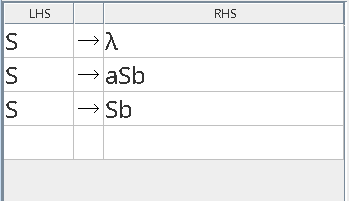
\includegraphics[width=\textwidth]{./Imagenes/produccion1.png}
                        \caption{la producción}
                        \label{fig:label1}
                    \end{subfigure}
                    \hfill
                    \begin{subfigure}[b]{0.45\textwidth}
                        \centering
                        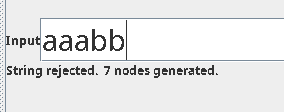
\includegraphics[width=\textwidth]{./Imagenes/grafoaaabb.png}
                        \caption{la cadena $aaabb$}
                        \label{fig:label2}
                    \end{subfigure}
                    \vspace{0.5cm} 
                    \\
                    \begin{subfigure}[b]{0.45\textwidth}
                        \centering
                        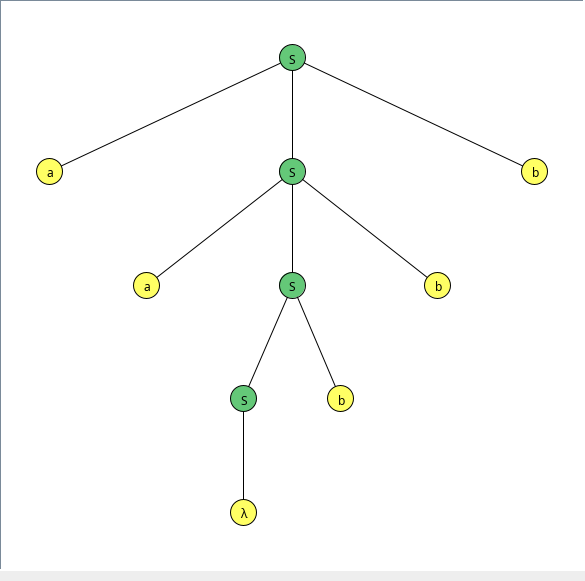
\includegraphics[width=\textwidth]{./Imagenes/grafoaabbb.png}
                        \caption{la cadena $aabbb$}
                        \label{fig:label3}
                    \end{subfigure}
                    \hfill
                    \begin{subfigure}[b]{0.45\textwidth}
                        \centering
                        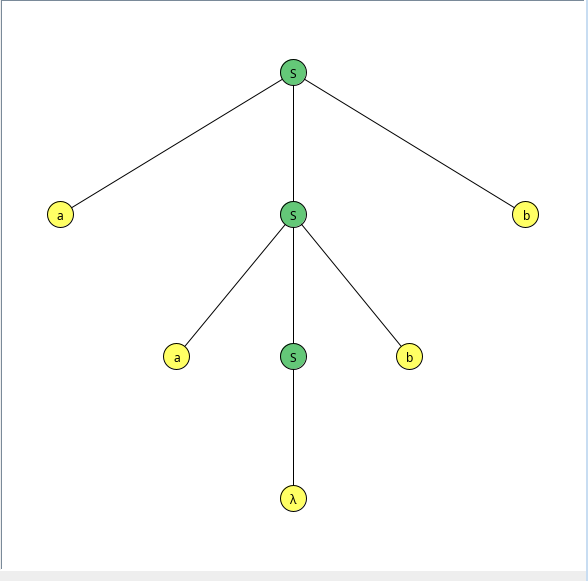
\includegraphics[width=\textwidth]{./Imagenes/grafoaabb.png}
                        \caption{la cadena $aabb$}
                        \label{fig:label4}
                    \end{subfigure}
                    \label{fig:matrix}
                \end{figure}

                    
                    
                

            \end{enumerate}
        \end{flushleft}


    \end{document}
